% Human computation e GWAP
% cos'è

Computers are capable of performing many tasks, they can process large
amounts of data and do billions of operation in a few seconds.
However, there are still many problems that computers cannot solve
or take too much time to solve even for the powerful pc.\\

Some of these are very simple tasks for humans, for example natual language
processing and object regonition are hard to solve problem for a computer
but natural for a human being. A great example for this kind of problem
is recognizing hand-written text, even after years of research,
humans are still faster and more accurate than any computer.\\

Furthermore, there are problems that are too computationally expensive,
such as many NP-complete problems like Traveling Salesman problem,
scheduling problems, packing problems, and FPGA routing problems.\\

The expression \emph{Human Computation} in the context of computer
science is already used by \cite{cogprints499}. However is \cite{human:comp}
to introduce the modern usage of the term. He defines human computation
as \emph{a research area of computer science that aims to build systems allowing
massive collaboration between humans and computers to solve problems that
could be impossible for either to solve alone}. But, in my opinion simple
and direct definitions are better to get the point:
\begin{quoting}
	Some problems are hard, even for the most\\
	sophisticated AI algorithms.\\
	Let humans solve it\omissis\\
	\medskip
    {\rm --- Edith Law}
\end{quoting}

% come è caratterizzata dal punto di vista pratico (come funziona)
% infrastrutture di esempio MTurk
In pratice when speaking about human computation we refer to an algorithm that
involves humans interaction during the computational process. As an example
infrastructure one can think of \citetitle{turk}, a \emph{centralized} human
computation platform that leverage on \emph{Workers} to perform task.

% categorizzazione in centralizzato e distribuito
By using the term \emph{centralized} we mean that all the computation is
performed in one \underline{central} place (e.g. \citetitle{turk} website). On
the other hand we have \emph{distributed} human computation, here the code
is offloaded to the client using some ad-hoc software clients.







\subsubsection{Centralized}
% il codeice viene eseguito su un sito non viene scaricata sul client (offload)
% Mturk, ESP, Crowd search
The \emph{centralized} paradigm is the most common because it do not require the
creation of ad-hoc clients to perform computation, that can run directly in the
browser. Now we present some of the well known online tools that use this kind
of algorithm.

\paragraph{\citetitle{turk}} is an online tool that allow the execution of
crowd-based human computation task, called \ac{HIT}. Each \ac{HIT} is created
by a \emph{Requester} whom decides also the revenue for the execution of the
tasks and some other constraints to the execution (i.e. user qualification).
Once the creation is completed the \ac{HIT} is ready to be executed by a
\emph{Worker}. A \emph{Worker} is a human being registered to the \citetitle{turk}
platform willing to perform simple task in exchange for money, the revenews can
be as low as 0.01\$ per user per task. Once the whole \ac{HIT} is completed the
\emph{Requester} check the result and if it is satisfied proceed with the
payment. All these operation must be performed within the \citetitle{turk}
website so there is no need of any software installed.\\
\begin{figure}[htb]
    \centering
    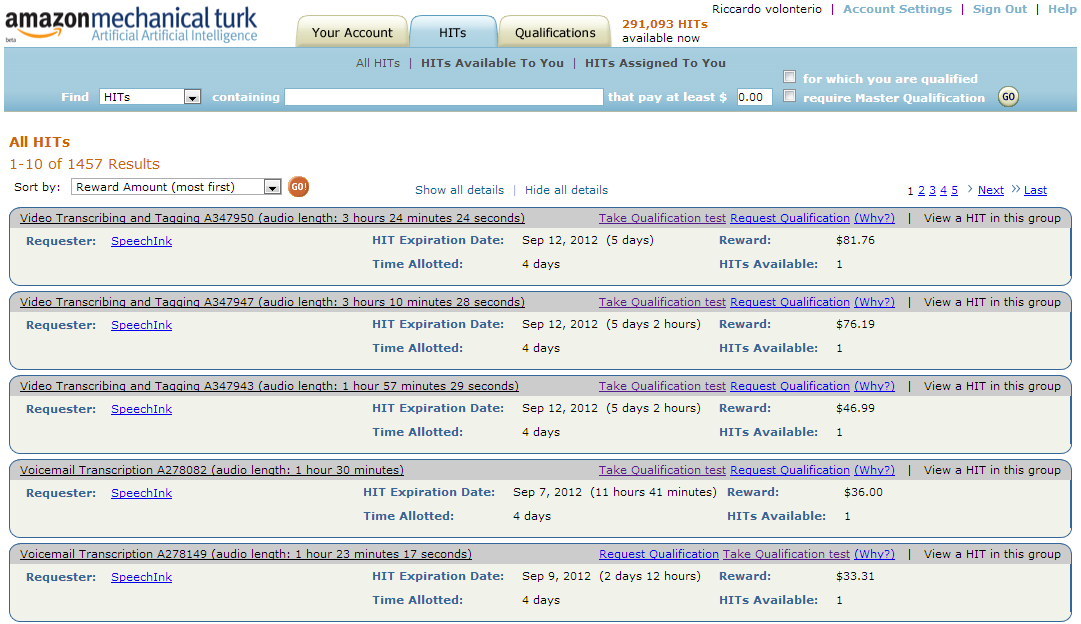
\includegraphics[width=\columnwidth]{turk}
    \caption{Web interface of \citetitle{turk}.}
    \label{fig:turk}
\end{figure}

This system has been \emph{extended} as presented in \cite{little2010turkit}
to create complete algorithm able to use human computation as functions during
the execution. Here is an example algorithm implemented in Turkit:
\begin{lstlisting}[language=C++]
ideas = []
for (var i = 0; i < 5; i++) {
	idea = mturk.prompt("What's fun to see in New York City? Ideas so far: " + ideas.join(", "))
	ideas.push(idea)
}
ideas.sort(function (a, b) {
	v = mturk.vote("Which is better?", [a, b])
	return v == a ? -1 : 1
})
\end{lstlisting}
Where \code{mturk.prompt} and \code{mturk.vote} are human computation task
executed on the \citetitle{turk} platform.

\paragraph{ESP} is a \ac{GWAP} developed by Luis von Ahn to perform image
their task is to agree on a word that would be an appropriate label for the
recognition using the power of humans as described in \cite{von2004labeling}.
The game rules are simple, once logged in a user will be automatically matched
with a random partner. Once matched, they will both be shown the same image,
their task is to agree on a word that would be an appropriate label for the
image. Similar to the ESP game is Peekaboom another \ac{GWAP} proposed by von
Ahn described in \cite{von2006peekaboom}.
\begin{figure}[htb]
    \centering
    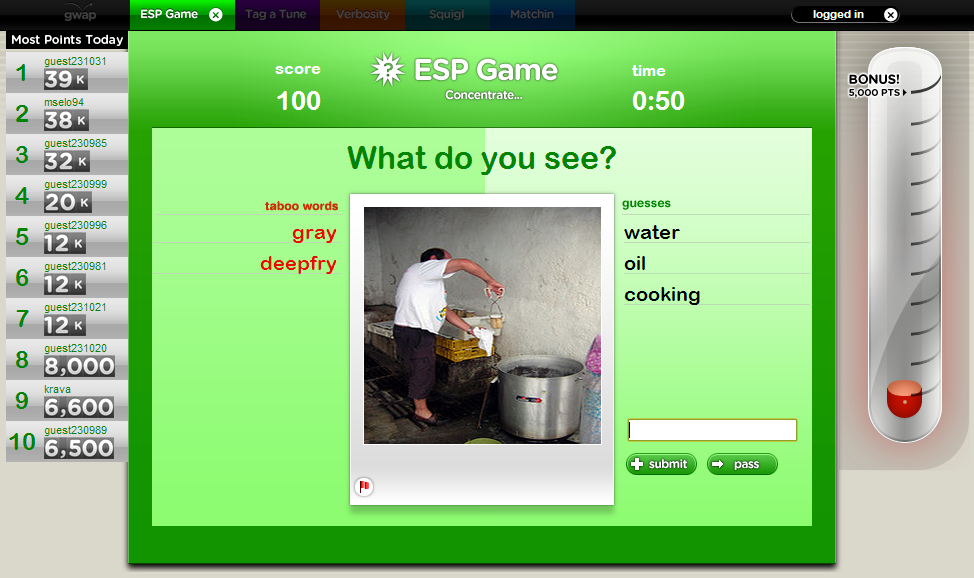
\includegraphics[width=0.75\columnwidth]{esp}
    \caption{The ESP game.}
    \label{fig:esp}
\end{figure}


\paragraph{CrowdSearcher}
TODO ???






\subsubsection{Distributed}
This solution relies on the creation of ad-hoc clients that are able to download
and run the code on all the platforms. With this solution the user do not need
to go to a website to run the code remotely. The most known implementation of
this paradigm is the \citetitle{foldit} game.\\

\paragraph{\citetitle{foldit}} is a puzzle game about protein folding, developed
by the University of Washington's Center for Game Science in collaboration with
the UW Department of Biochemistry. The objective of the game is to fold the
structure of selected proteins to the best of the player's ability. The highest
scoring solutions are analysed by researchers, that can determine whether or not
there is a native structural configuration that can be applied to the relevant
proteins.
\begin{figure}[htb]
    \centering
    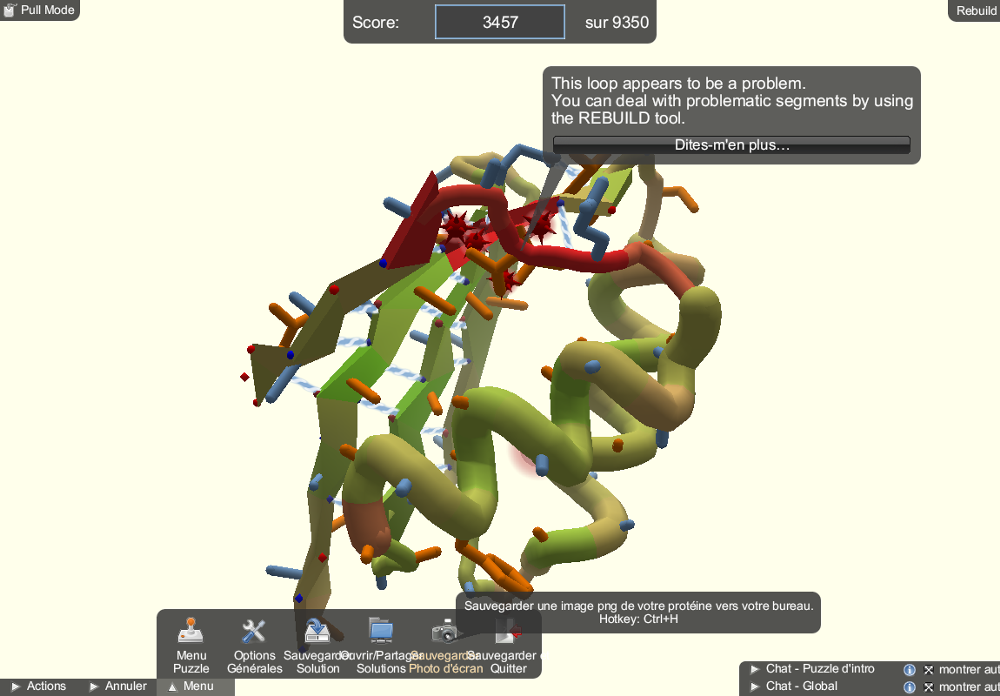
\includegraphics[width=\columnwidth]{foldit}
    \caption{The FoldIt client.}
    \label{fig:foldit}
\end{figure}